\documentclass[conference]{IEEEtran}

% Packages
\usepackage[utf8]{inputenc}
\usepackage[english]{babel}
\usepackage{amsmath}
\usepackage{amsfonts}
\usepackage{amssymb}
\usepackage{amsthm}
\usepackage{pdfpages}
\usepackage{graphicx}
\usepackage{epstopdf}
\usepackage{listings}
\usepackage{cite}
\usepackage{enumerate}
\usepackage{scientific}
\usepackage[colorlinks=false]{hyperref}
\usepackage{bookmark}
\usepackage{paralist}

\usepackage[]{mcode}	%Matlab Code
\usepackage{tikz,pgfplots}	%Tikz

%\usepgfplotslibrary{external} 
%\tikzexternalize
%\tikzsetexternalprefix{ext/}

% Bookmark Setup
\bookmarksetup{numbered}

% PDF Setup
\hypersetup{pdftitle={Homework 7}, pdfsubject={Documentation of 7th Homework}, pdfauthor={Stefan Röhrl}, pdfkeywords={Neuroprothetik Exercise}, pdfcreator={LaTeX}, hidelinks}


\begin{document}
%
% cite all references
%\nocite{*}
%
% paper title
% can use linebreaks \\ within to get better formatting as desired
\title{Homework 8\\ Einhüllende \& nicht lineare Dynamik Kompression}

\author{\IEEEauthorblockN{Stefan Röhrl}
\IEEEauthorblockA{Technische Universität München, Arcisstraße 21, Munich, Germany\\
Email: stefan.roehrl@tum.de}}

% use for special paper notices
%\IEEEspecialpapernotice{(Invited Paper)}

%\onecolumn

% make the title area
\maketitle

\IEEEpeerreviewmaketitle

\section{Einhüllende}
\begin{compactenum}[a)]
\begin{figure}[h!]
	\vspace{-5pt}
	\centering
	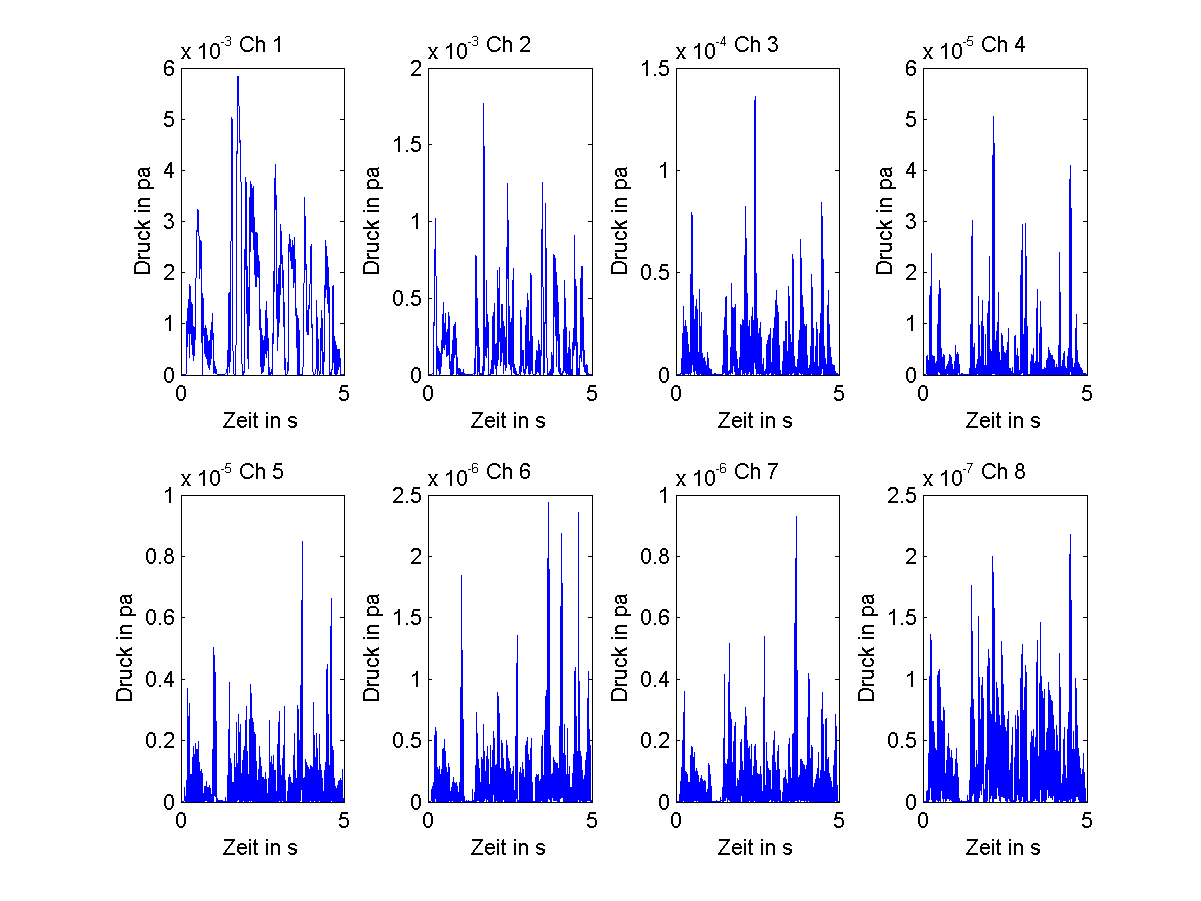
\includegraphics[width=0.5\textwidth]{img/env8.png}
	\vspace{-10pt}
	\caption{Einhüllende von 8 Kanälen}
	\vspace{-10pt}
	\label{fig:env8}
\end{figure}

\begin{figure}[h!]
	\vspace{-5pt}
	\centering
	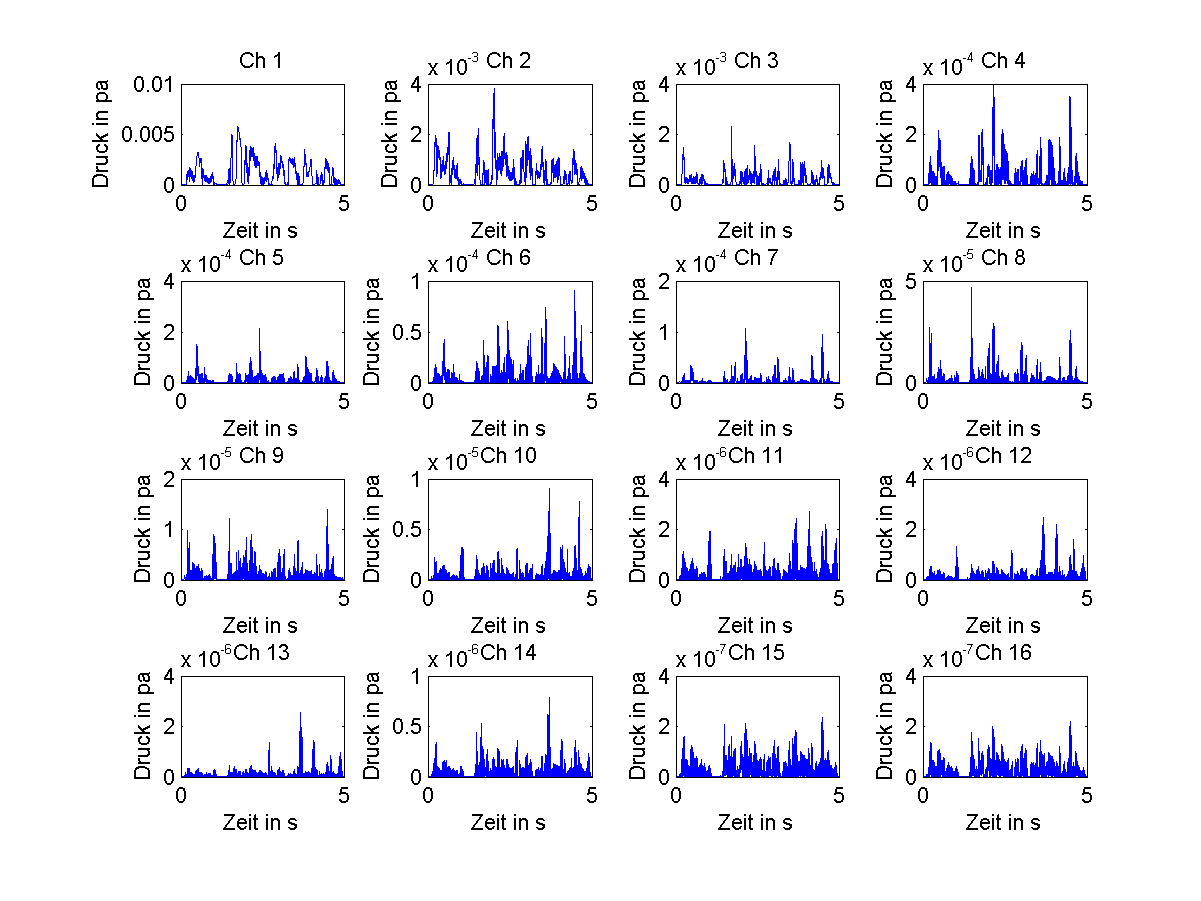
\includegraphics[width=0.5\textwidth]{img/env16.png}
	\vspace{-10pt}
	\caption{Einhüllende von 16 Kanälen}
	\vspace{-10pt}
	\label{fig:env16}
\end{figure}
\item Das zu verarbeitende Sprachsignal enthält folgenden englischen Satz: \textit{In language infinitely many words can be written with a small set of letters}. Dieses Signal wurde zuerst mit einer 8- bzw. 16-Kanal-Filterbank in unterschiedliche Frequenzbänder aufgeteilt. Von den Ausgängen jedes Kanals wurden mit der Hilbert Transformation die Einhüllenden des Signal berechnet. Die jeweiligen Einhüllenden für jeden Kanal der beiden Filterbänke sind in Abbildung \ref{fig:env8} und \ref{fig:env16} zu sehen. Auffällig ist das Kanäle für tiefe Frequenzen einen weitaus höheren Pegel aufweisen, als Kanäle für hohe Frequenzen. 

\newpage
\item In Abbildung \ref{fig:sig_orig} ist das originale Zeitsignal zu erkennen, welches eine Ausdehnung von 5 Sekunden hat. Darunter in Abbildung \ref{fig:freq_orig} ist das komplette Frequenzspektrum des unveränderten Signals zu sehen. Da es sich um ein menschliches Sprachsignal handelt, liegen die Frequenzanteile zwischen 100 und ca. 8kHz. 
\begin{figure}[h!]
	\vspace{-5pt}
	\centering
	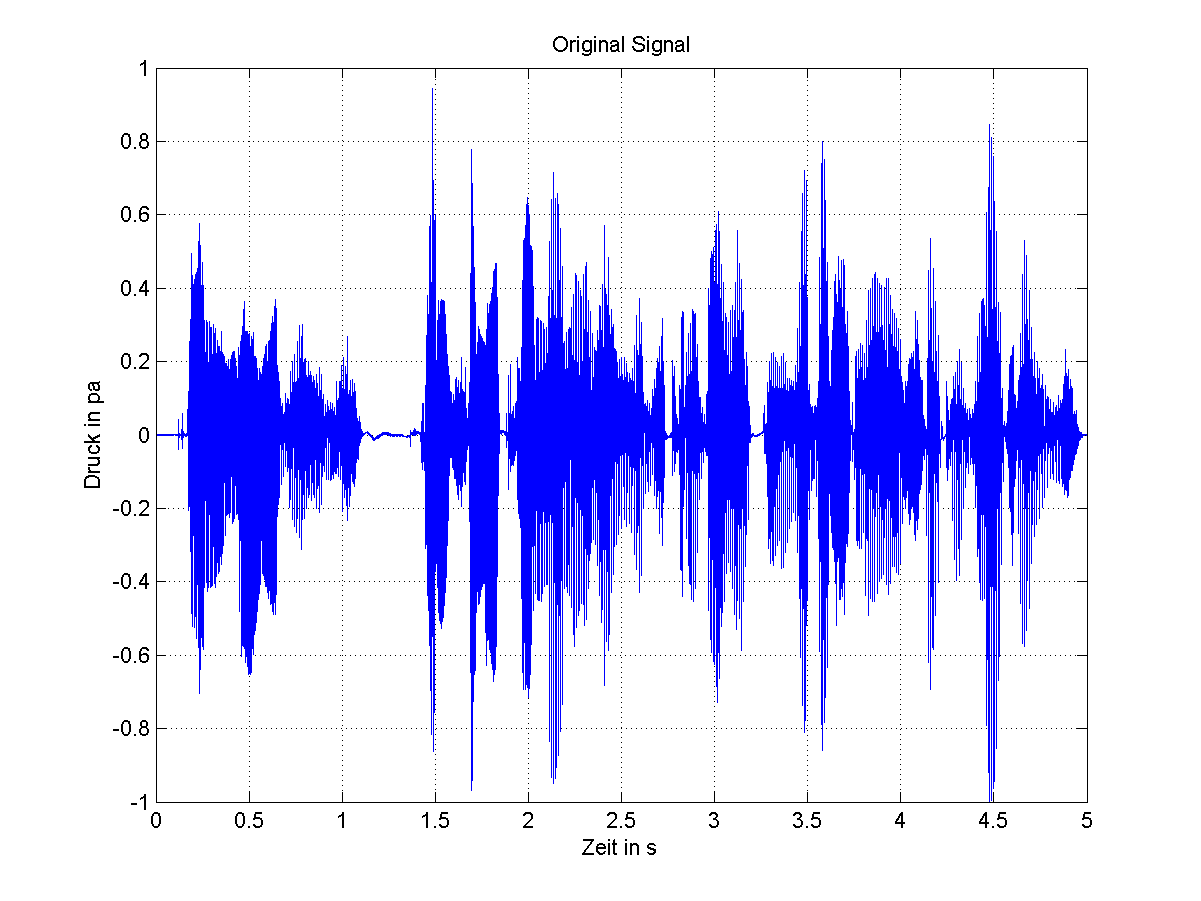
\includegraphics[width=0.5\textwidth]{img/sig_orig.png}
	\vspace{-20pt}
	\caption{Original Signal}
	\vspace{-10pt}
	\label{fig:sig_orig}
\end{figure}
\begin{figure}[h!]
	\vspace{-5pt}
	\centering
	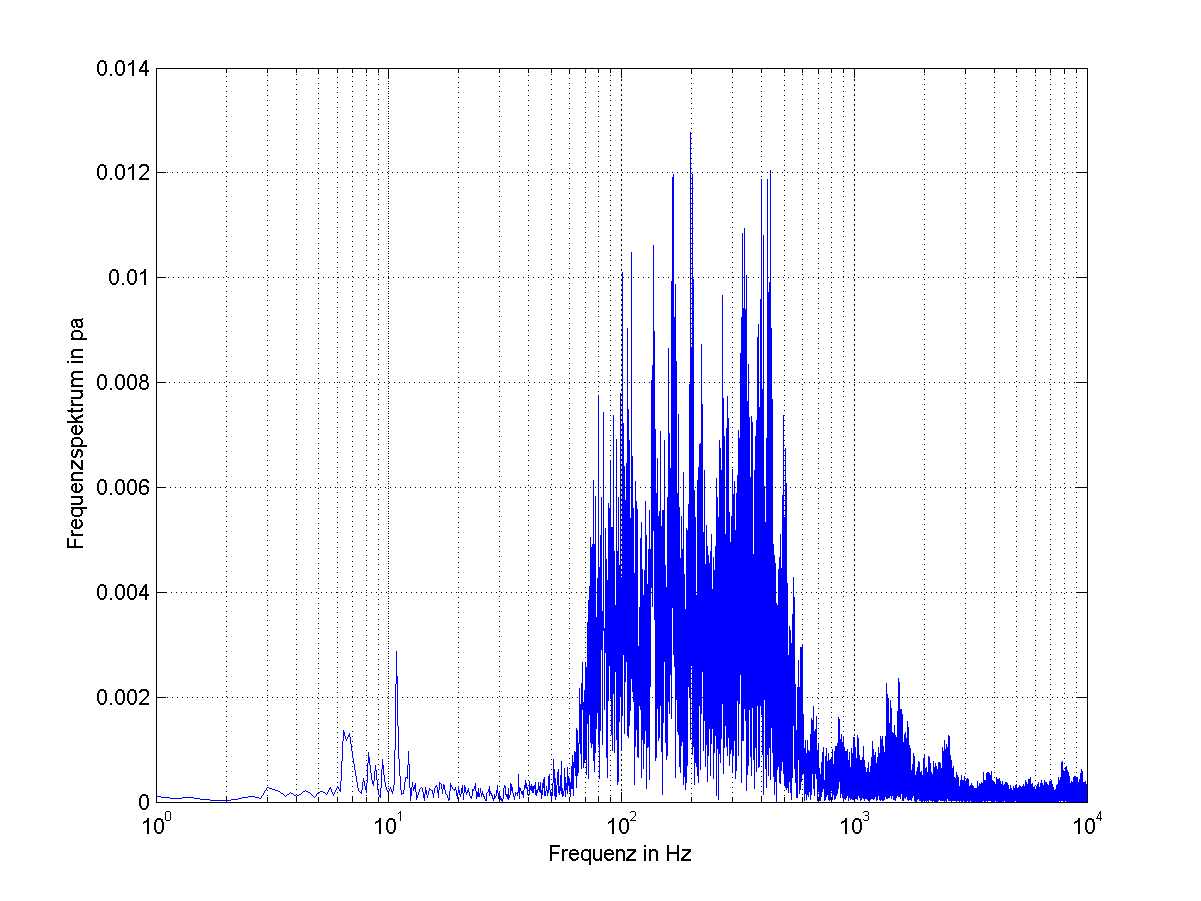
\includegraphics[width=0.5\textwidth]{img/freq_orig.png}
	\vspace{-20pt}
	\caption{Frequenzspektrum Original Signal}
	\vspace{-10pt}
	\label{fig:freq_orig}
\end{figure}
Das Kurzzeit-Sektprogramm zeigt die Frequenzanteile nicht komplett für den ganzen Signalverlauf sondern immer für den jeweiligen Zeitabschnitt im Signal. Auch hier sieht man wieder die Unterschiede zwischen dem original Signal und den gefilterten Signalen. Man muss jedoch beachten, das es sich bei den Signalen aus der Filterbank nur noch um die Einhüllenden des Signals handelt und diese nicht direkt mit dem original Signal vergleichbar sind. Man sieht jedoch auch wieder deutlich die höhere Frequenzauflösung der 16-Kanal-Filterbank im Gegensatz zur 8-Kanal-Filterbank. Des weiteren fällt auf, dass die Kanäle nicht richtig ausgelastet sind, nur wenige Stellen sind heller gefärbt als dunkelblau. Dies soll mit einer Dynamikkompression verbessert werden.
\begin{figure}[h!]
	\vspace{-5pt}
	\centering
	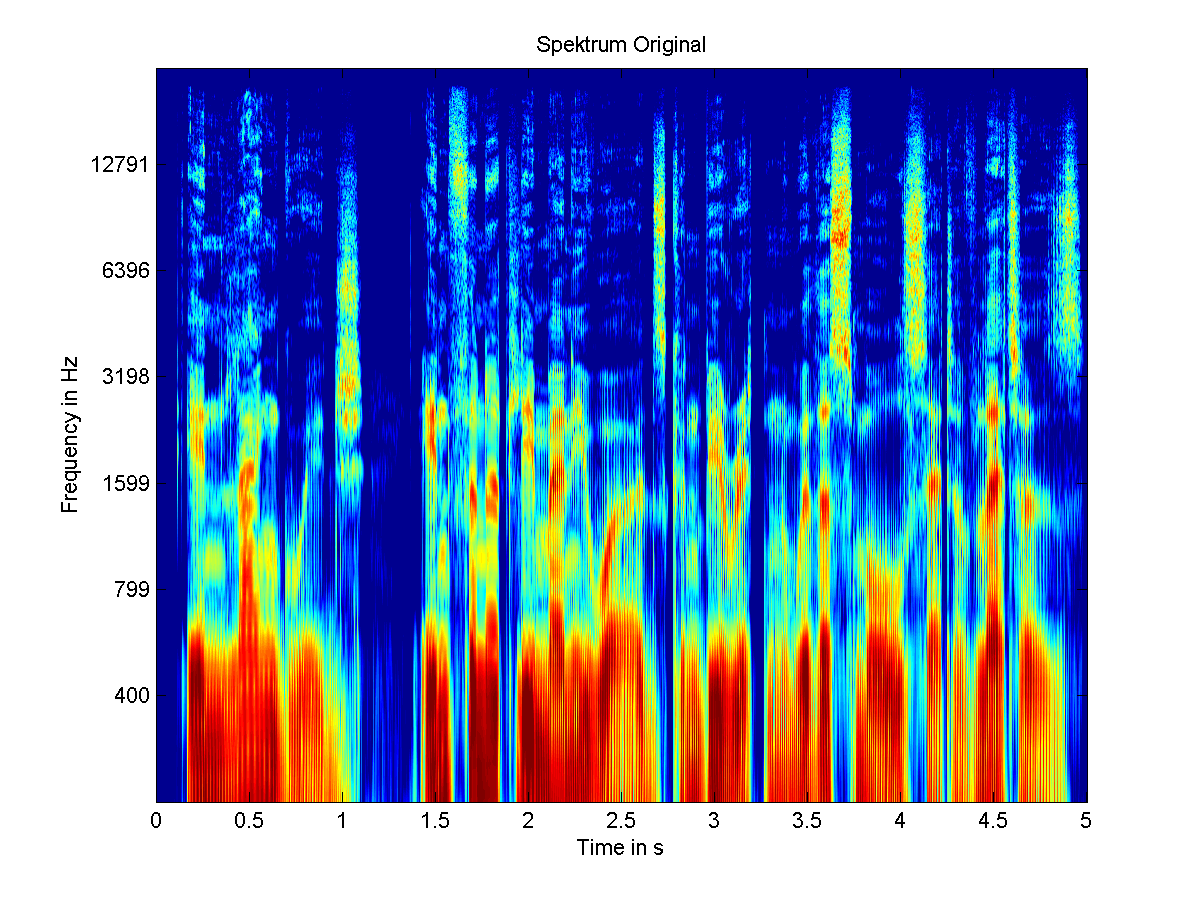
\includegraphics[width=0.5\textwidth]{img/spec_orig.png}
	\vspace{-10pt}
	\caption{Kurzzeit-Spektrogramm Original Signal}
	\vspace{-10pt}
	\label{fig:spec_orig}
\end{figure}
\begin{figure}[h!]
	\vspace{-5pt}
	\centering
	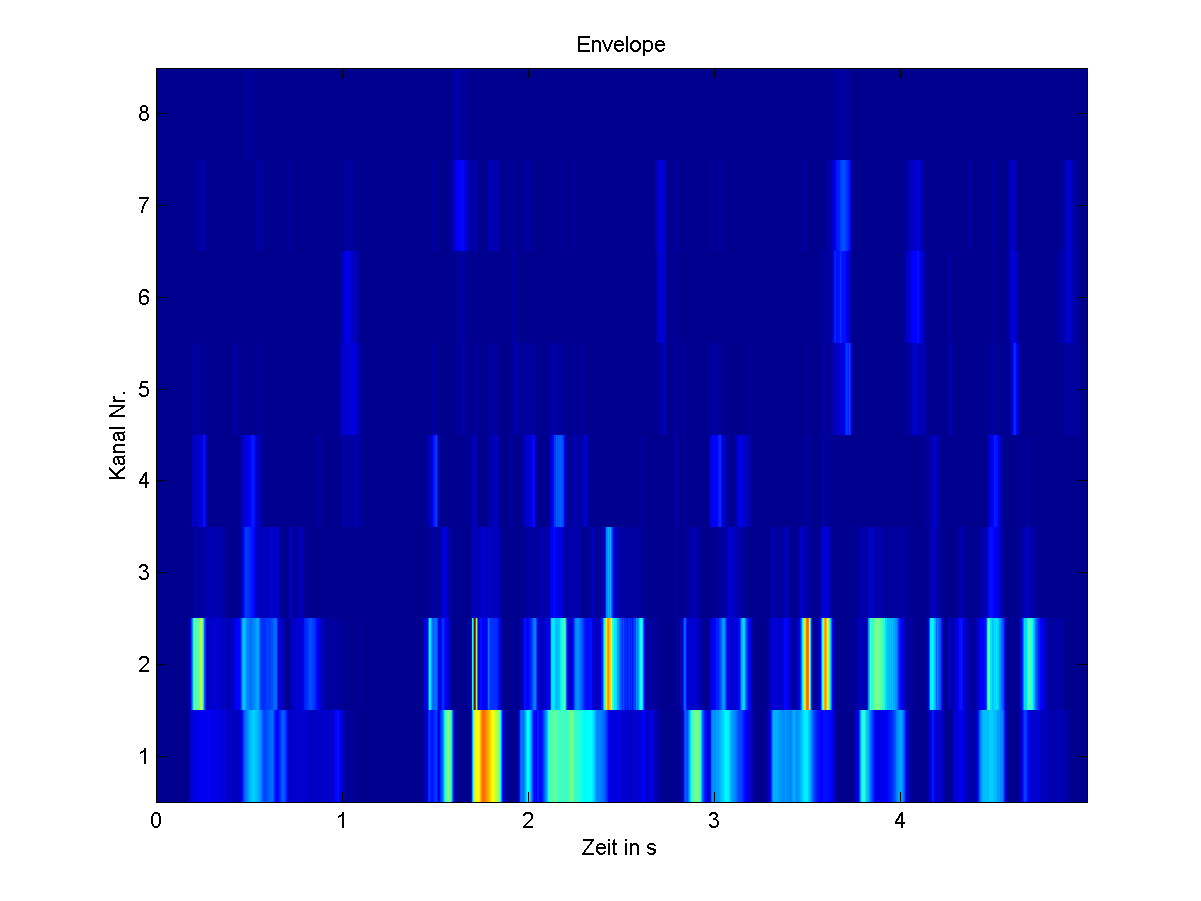
\includegraphics[width=0.5\textwidth]{img/spec_env8.png}
	\vspace{-10pt}
	\caption{Kurzzeit-Spektrogramm der Einhüllenden mit 8 Kanälen}
	\vspace{-10pt}
	\label{fig:spec_env8}
\end{figure}
\begin{figure}[h!]
	\vspace{-5pt}
	\centering
	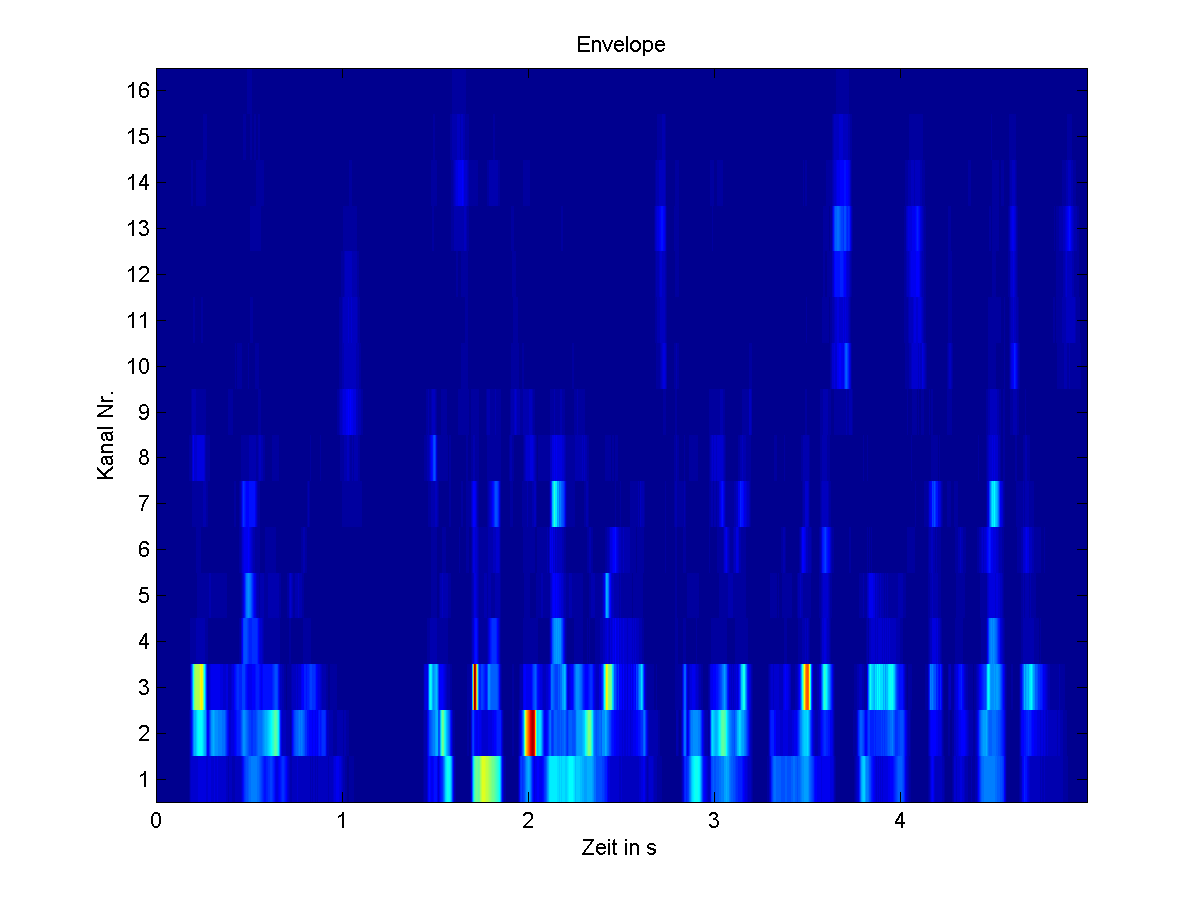
\includegraphics[width=0.5\textwidth]{img/spec_env16.png}
	\vspace{-10pt}
	\caption{Kurzzeit-Spektrogramm der Einhüllenden mit 16 Kanälen}
	\vspace{-10pt}
	\label{fig:spec_env16}
\end{figure}

\newpage
Das Summenspektrum zeigt den mittleren Pegel eines Kanals - also ein bestimmtes Frequenzband - über der Zeit. In diesem Spektrum kann man erkennen, dass besonders die hohen Frequenzen nur einen kleinen Anteil am Gesamtpegel haben. Dies ist sowohl bei der 8 und der 16-Kanal-Filterbank der Fall.
\begin{figure}[h!]
	\vspace{-5pt}
	\centering
	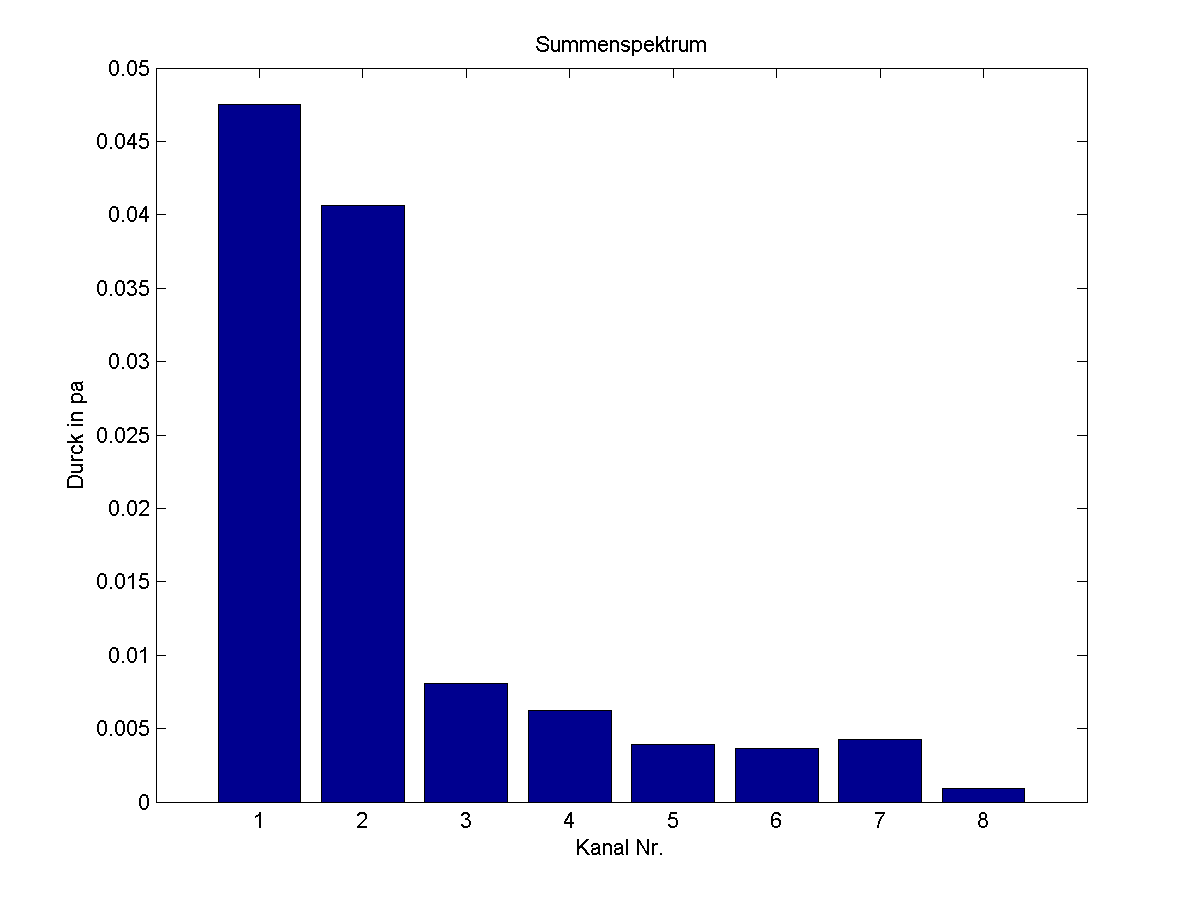
\includegraphics[width=0.5\textwidth]{img/sum_ch8.png}
	\vspace{-10pt}
	\caption{Summenspektrum der Einhüllenden mit 8 Kanälen}
	\vspace{-10pt}
	\label{fig:sum_env8}
\end{figure}

\begin{figure}[h!]
	\vspace{-5pt}
	\centering
	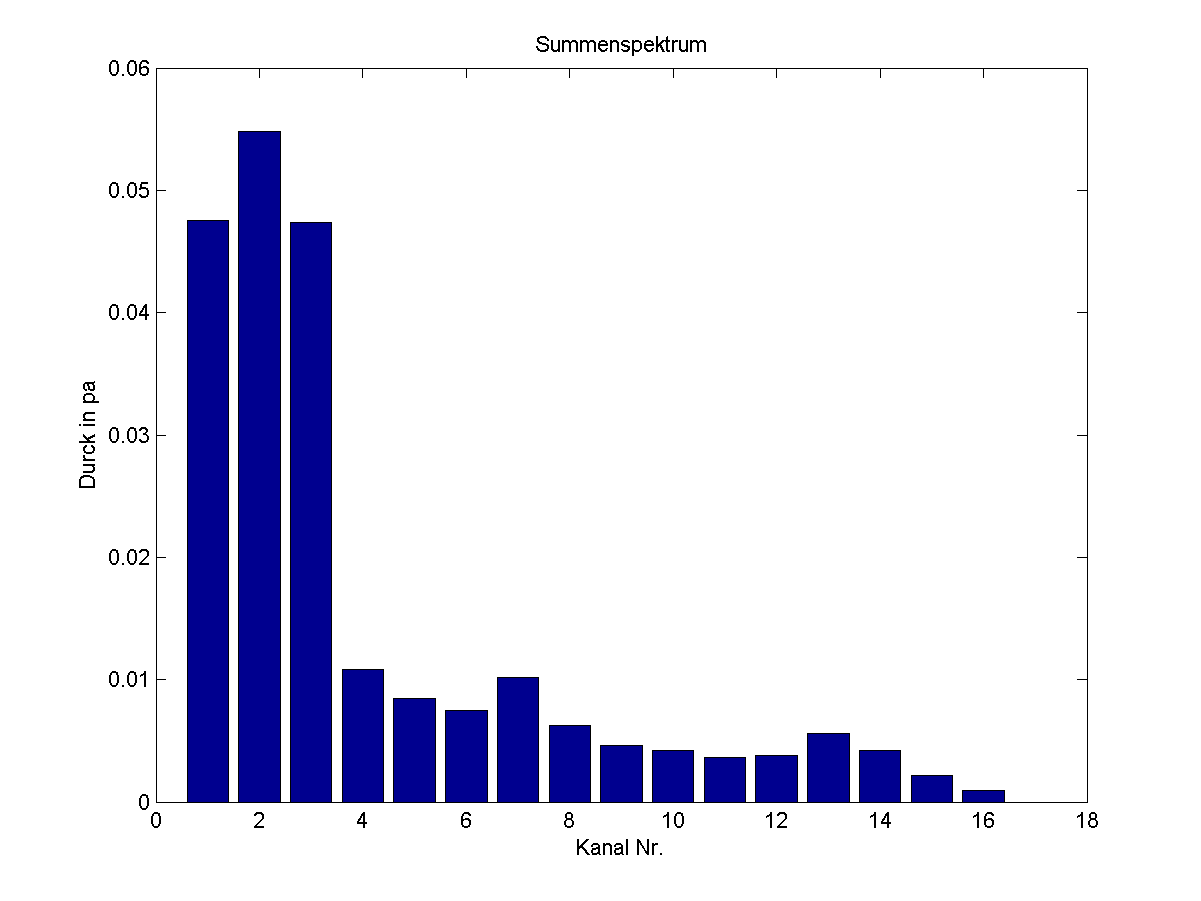
\includegraphics[width=0.5\textwidth]{img/sum_ch16.png}
	\vspace{-10pt}
	\caption{Summenspektrum der Einhüllenden mit 16 Kanälen}
	\vspace{-10pt}
	\label{fig:sum_env8}
\end{figure}
\end{compactenum}

\clearpage
\section{Dynamikkompression}
\begin{compactenum}[a)]
\item Da das gesprochene Signal einen ziemlich großen Dynamikbereich hat, welcher so nur schlecht zu kodieren ist, wird eine nicht lineare Dynamikkompression vorgenommen. Diese verstärkt leise Signale mehr als bereits laute Signale. Somit ist der unterschied zwischen lauten und leisen Abschnitten nicht mehr so groß und es muss nur noch ein kleinerer Lautstärkebereich abgebildet werden. Nach der Dynamikkompression befinden sich die Pegel der Einhüllenden alle in der Größenordnung $10^{-3}$ Pa (vgl. Abb. \ref{fig:dyn8} und \ref{fig:dyn16}). Nicht so wie vor der Dynamikkompression, wo Kanäle mit niedrigen Frequenzen Pegel in der Größenordnung von $10^{-1}$ Pa aufweisen und Kanäle mit hohen Frequenzen im Bereich von $10^{-7}$ Pa arbeiten (vgl. Abb. \ref{fig:env16}).
\begin{figure}[h!]
	\vspace{-5pt}
	\centering
	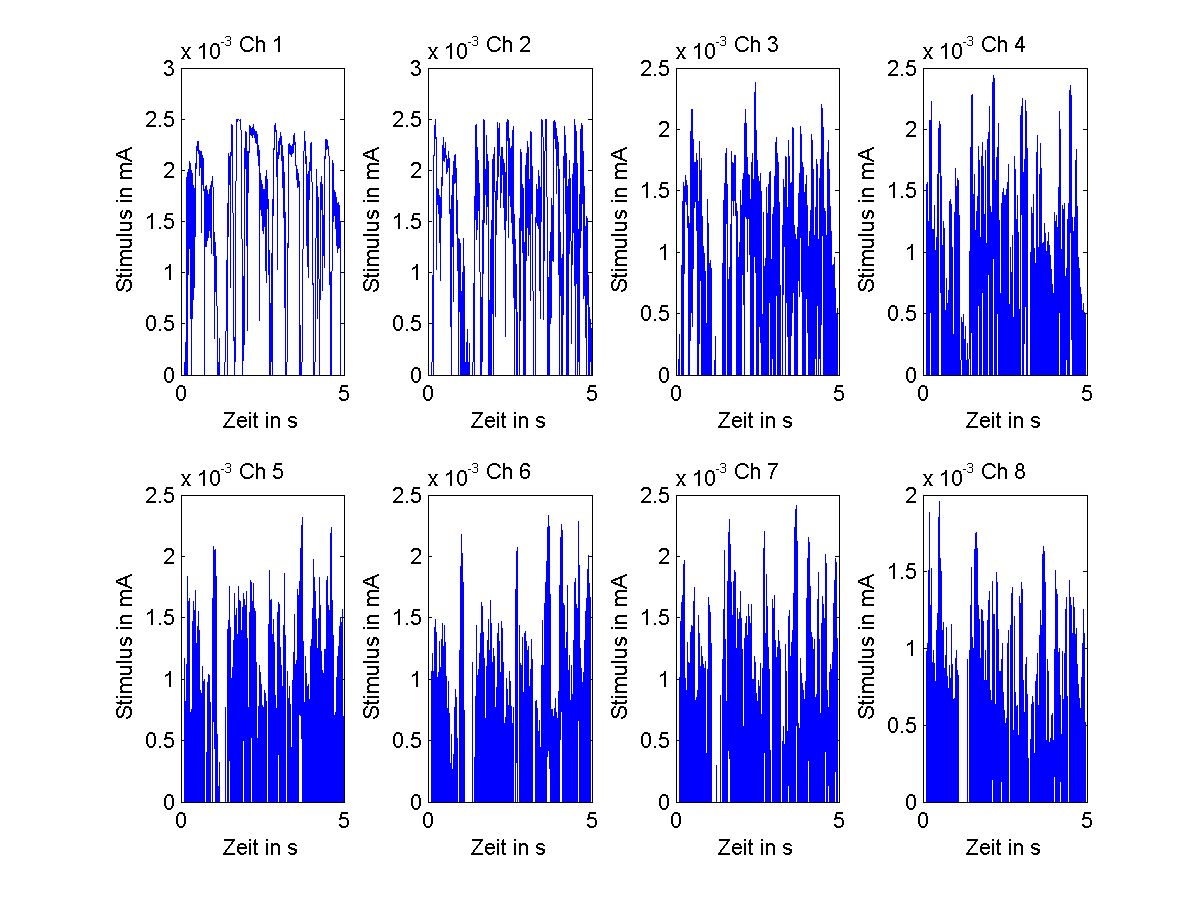
\includegraphics[width=0.5\textwidth]{img/dyn8.png}
	\vspace{-10pt}
	\caption{Einhüllenden mit Dynamikkompression von 8 Kanälen}
	\vspace{-10pt}
	\label{fig:dyn8}
\end{figure}

\begin{figure}
	\vspace{-5pt}
	\centering
	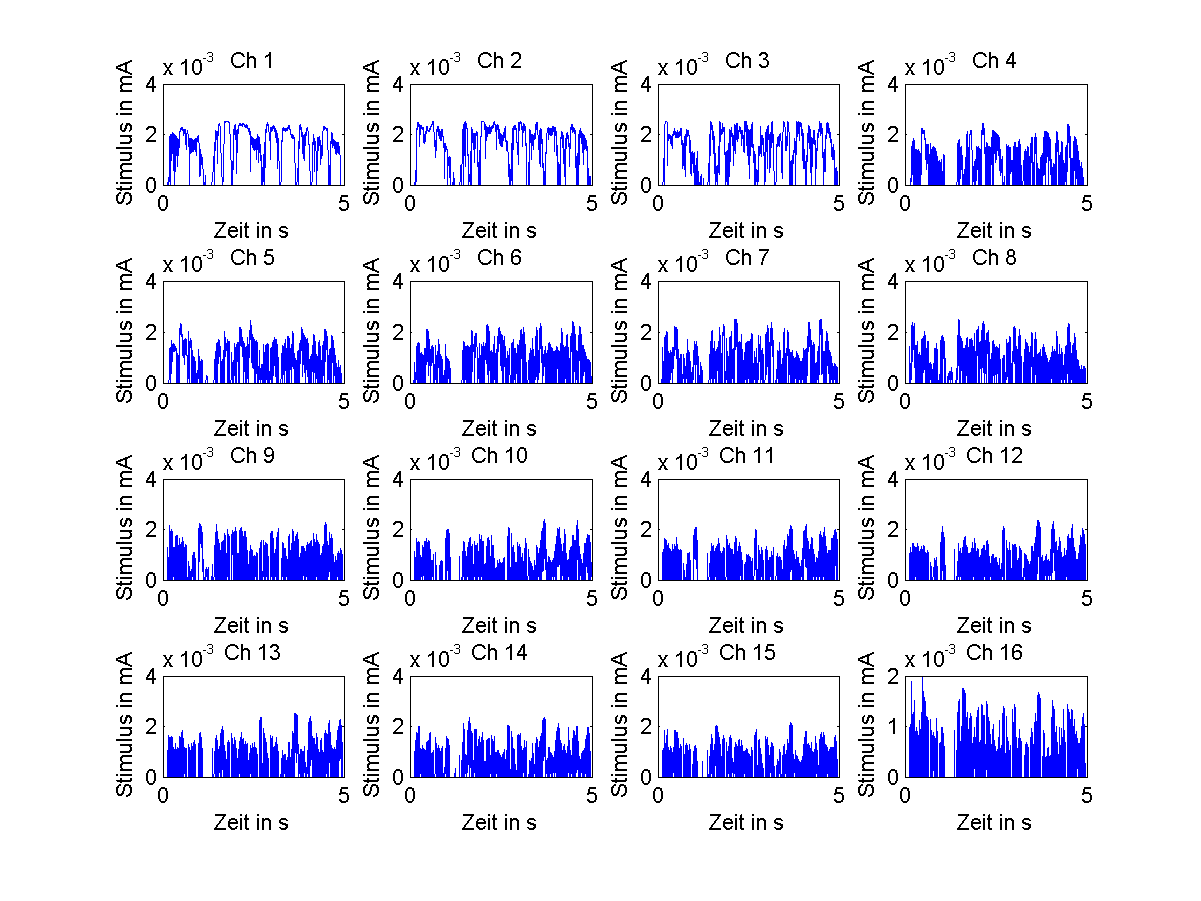
\includegraphics[width=0.5\textwidth]{img/dyn16.png}
	\vspace{-10pt}
	\caption{Einhüllenden mit Dynamikkompression von 16 Kanälen}
	\vspace{-10pt}
	\label{fig:dyn16}
\end{figure}

\newpage
\item Auch in den Kurzzeit-Spektrogrammen ist nun eine wesentlich höhere Auslastung zu erkennen. Da Pegel der verschiedenen Kanäle nun wesentlich näher beieinander liegen, kann man diese besser kodieren was sich eben auch in der Farbkodierung zeigt (vgl. Abb. \ref{fig:spec_dyn8} und \ref{fig:spec_dyn16}). Selbst die Kanäle mit hohen Frequenzen zeigen nun deutliche Pegel und das original Signal wird deutlich besser repräsentiert. Besonders die Darstellung mit 16 Kanälen ähnelt viel mehr dem Originalspektrum (vgl. Abb. \ref{fig:spec_orig}).
\begin{figure}
	\vspace{-5pt}
	\centering
	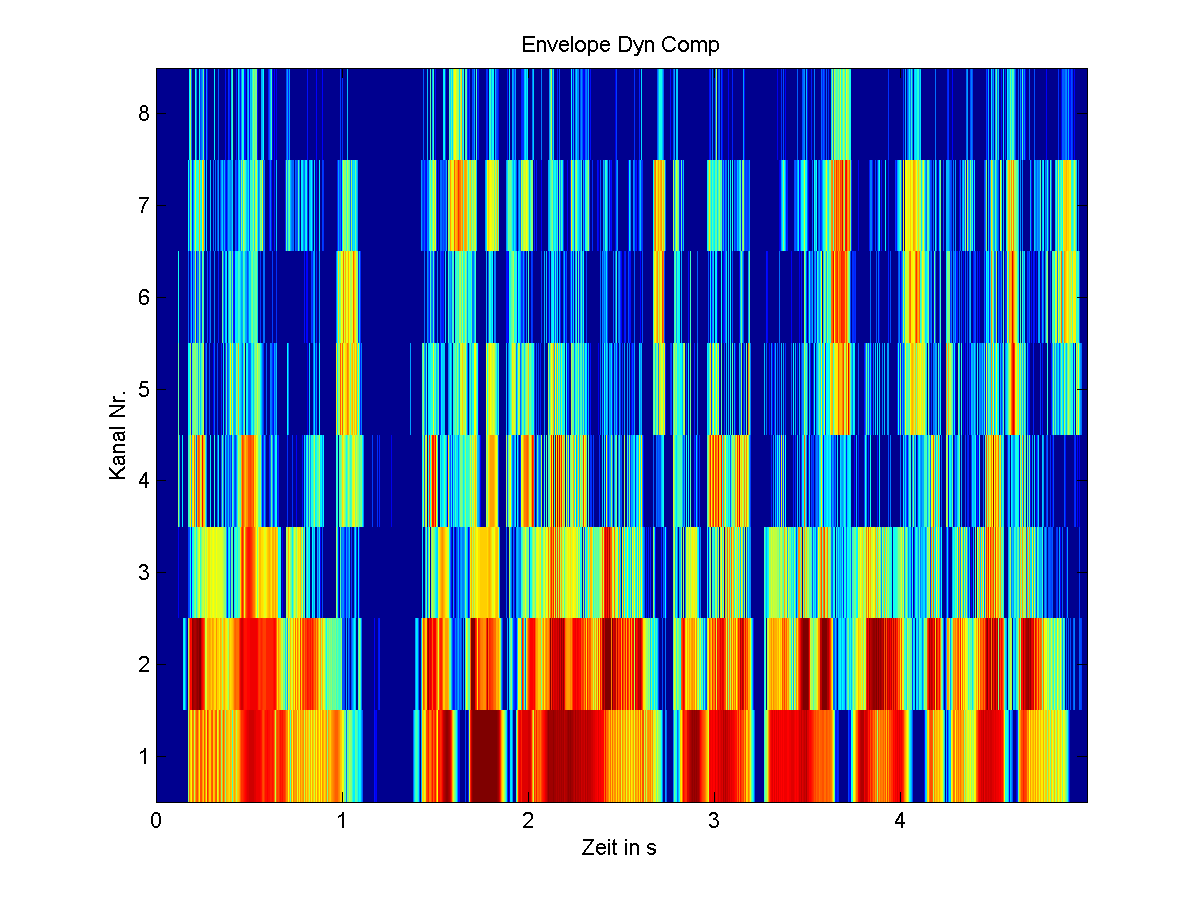
\includegraphics[width=0.5\textwidth]{img/spec_dyn8.png}
	\vspace{-10pt}
	\caption{Kurzzeit-Spektrogramm der Einhüllenden mit 8 Kanälen nach Dynamikkompression}
	\vspace{-10pt}
	\label{fig:spec_dyn8}
\end{figure}

\begin{figure}
	\vspace{-5pt}
	\centering
	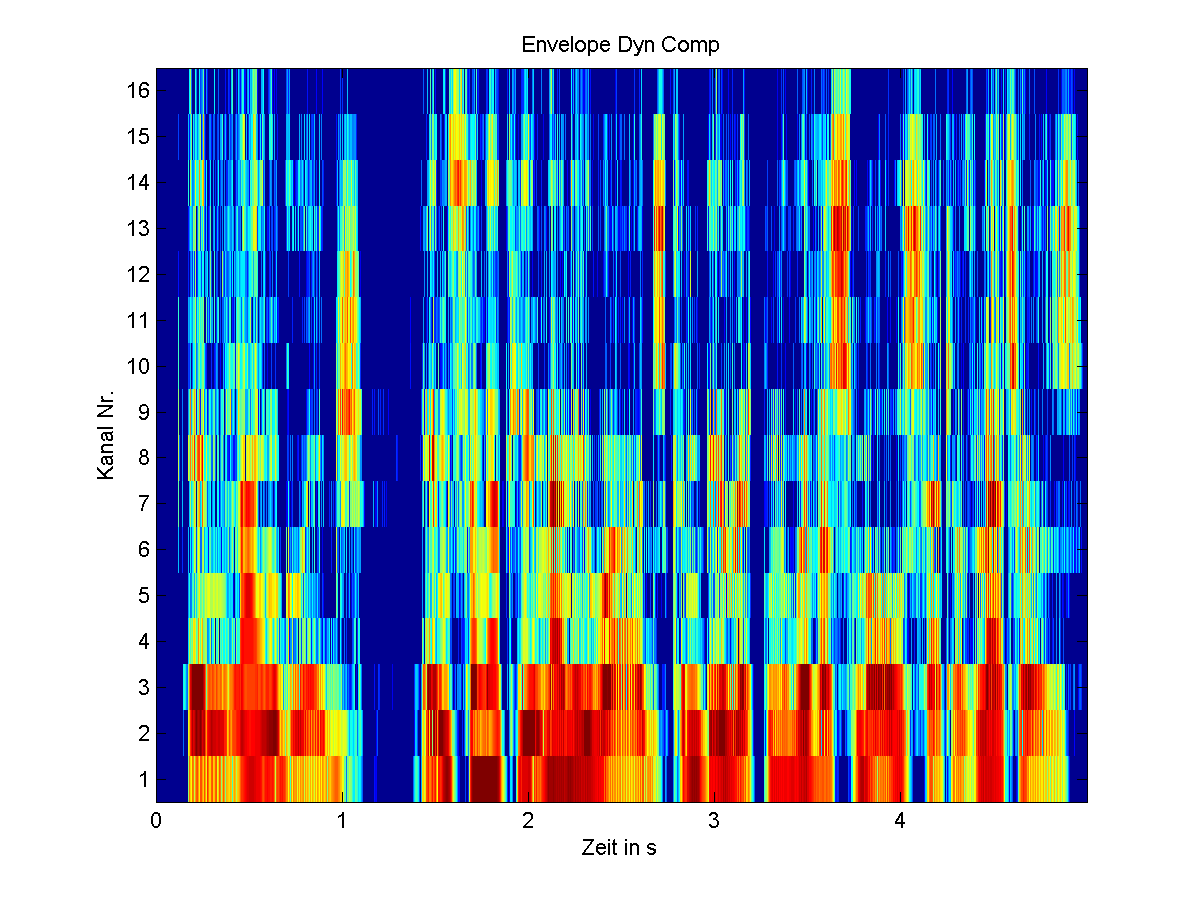
\includegraphics[width=0.5\textwidth]{img/spec_dyn16.png}
	\vspace{-10pt}
	\caption{Kurzzeit-Spektrogramm der Einhüllenden mit 16 Kanälen nach Dynamikkompression}
	\vspace{-10pt}
	\label{fig:spec_dyn16}
\end{figure}

\newpage
Auch in den Summenspektren sieht man eine deutliche Anhebung der hohen Frequenzen. Jedoch muss man auch feststellen, dass die Pegel der tiefen Frequenzbänder gestaucht wurden. Somit spielt sich der Dynamikbereich nur noch zwischen $10^{-3}$Pa und $10^{-4}$Pa ab, das heißt die Frequenzbänder liegen vom Pegel her auf ungefähr dem selben Level. Dies ermöglicht es die selbe Kodierung für alle Kanäle zu verwenden, ohne zu viele Informationen durch Clipping oder schlecht Auflösung in den niedrigen Bereichen zu bekommen. 
\begin{figure}
	\centering
	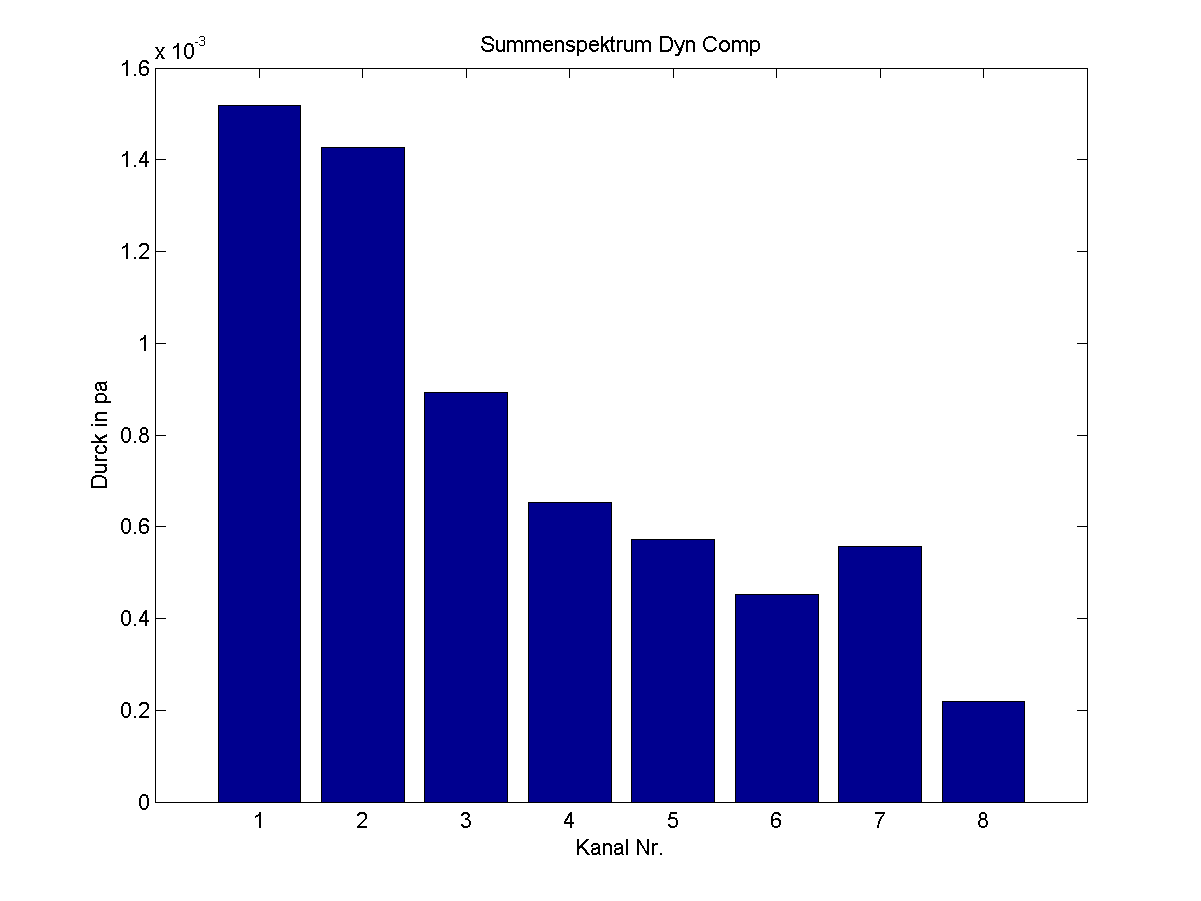
\includegraphics[width=0.5\textwidth]{img/sum_dyn8.png}
	\vspace{-10pt}
	\caption{Summenspektrum der Einhüllenden mit 8 Kanälen nach Dynamikkompression}
	\vspace{-10pt}
	\label{fig:sum_dyn8}
\end{figure}

\begin{figure}
	\centering
	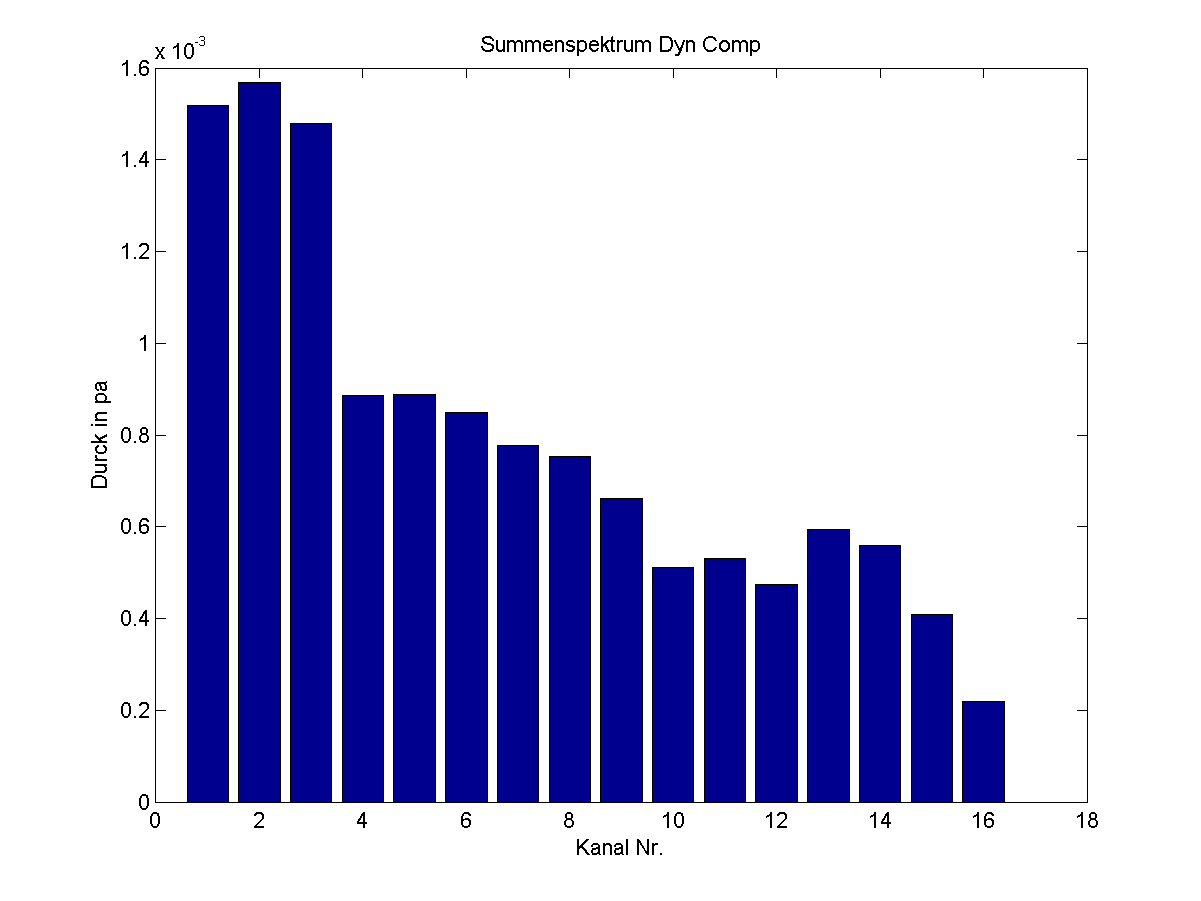
\includegraphics[width=0.5\textwidth]{img/sum_dyn16.png}
	\vspace{-10pt}
	\caption{Summenspektrum der Einhüllenden mit 16 Kanälen nach Dynamikkompression}
	\vspace{-10pt}
	\label{fig:sum_dyn16}
\end{figure}

\newpage
\item Das aufgenommene Signal muss für die Stimulation in Innenohr noch in eine Stromstärke umgerechnet werden. Die folgenden Abbildungen zeigen wie welche Schallpegel mit der vorher vorgenommenen Dynamikkompression in welche Stromstärken umgewandelt werden. Dabei sind die Abbildungen \ref{fig:lin_250} \ref{fig:lin_500} und \ref{fig:lin_1000} linear gezeichnet, wohingegen die Abbildungen \ref{fig:log_250} \ref{fig:log_500} und \ref{fig:log_1000} logarithmisch aufgetragen sind. Die Markierung $I_{MCL}$ steht für die höchste zulässige Stromstärke, die noch keine Schmerzen beim Patienten auslöst und somit nicht überschritten werden darf. Daher knickt die Kennlinie an dieser Stelle ab und es kommt zu Clipping. Die Markierung $I_{THR}$ steht für den minimalisiert möglichen Strom der kodiert werden kann. Signale mit kleinerem Pegel werden nicht ausgegeben. Alle Pegel dazwischen werden nicht-linear auf Stromstärken umgerechnet, wobei kleine Pegel mehr verstärkt werden als große. Es wurden drei verschiedene Kompressionsraten verwendet. Bei einer Kompressionsrate von 250 sieht man am logarithmischen Plot, dass sich die Kompression fast logarithmisch verhält, da im Plot eine Gerade zu sehen ist. Bei höheren Kompressionsraten wie 500 oder 1000 verhält sich die Kompression schon über-logarithmisch, da auch der logarithmische Plot keine Gerade mehr ist. Dies heißt hier werden kleine Pegel noch differenziert betrachtet und diesen ein nochmal weitaus größerer Dynamikbereich zur Verfügung gestellt, als den lauten Pegeln.
\newpage
\begin{figure}
	\centering
	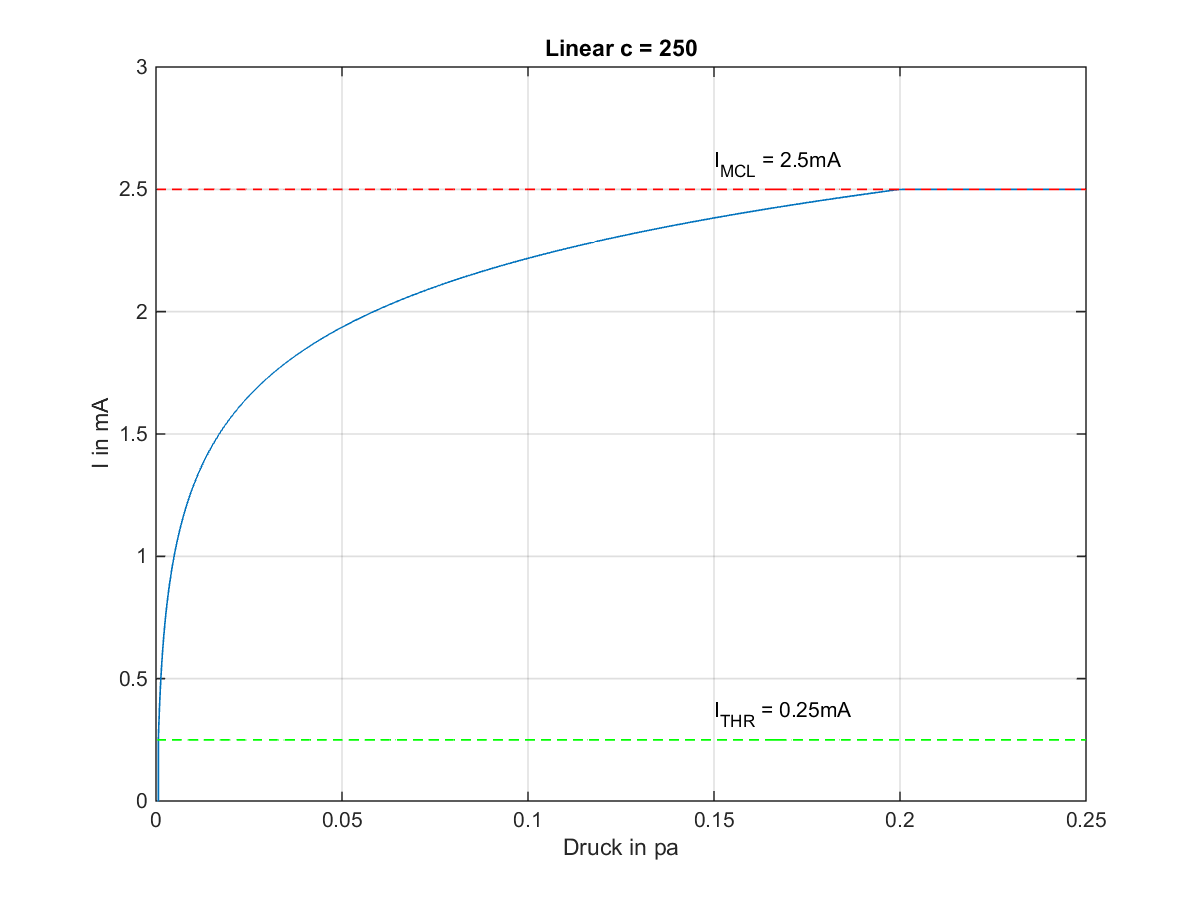
\includegraphics[width=0.5\textwidth]{img/lin_250.png}
	\vspace{-10pt}
	\caption{Kompressionskennlinie Linear mit Kompressionsrate 250}
	\vspace{-10pt}
	\label{fig:lin_250}
\end{figure}
\begin{figure}
	\centering
	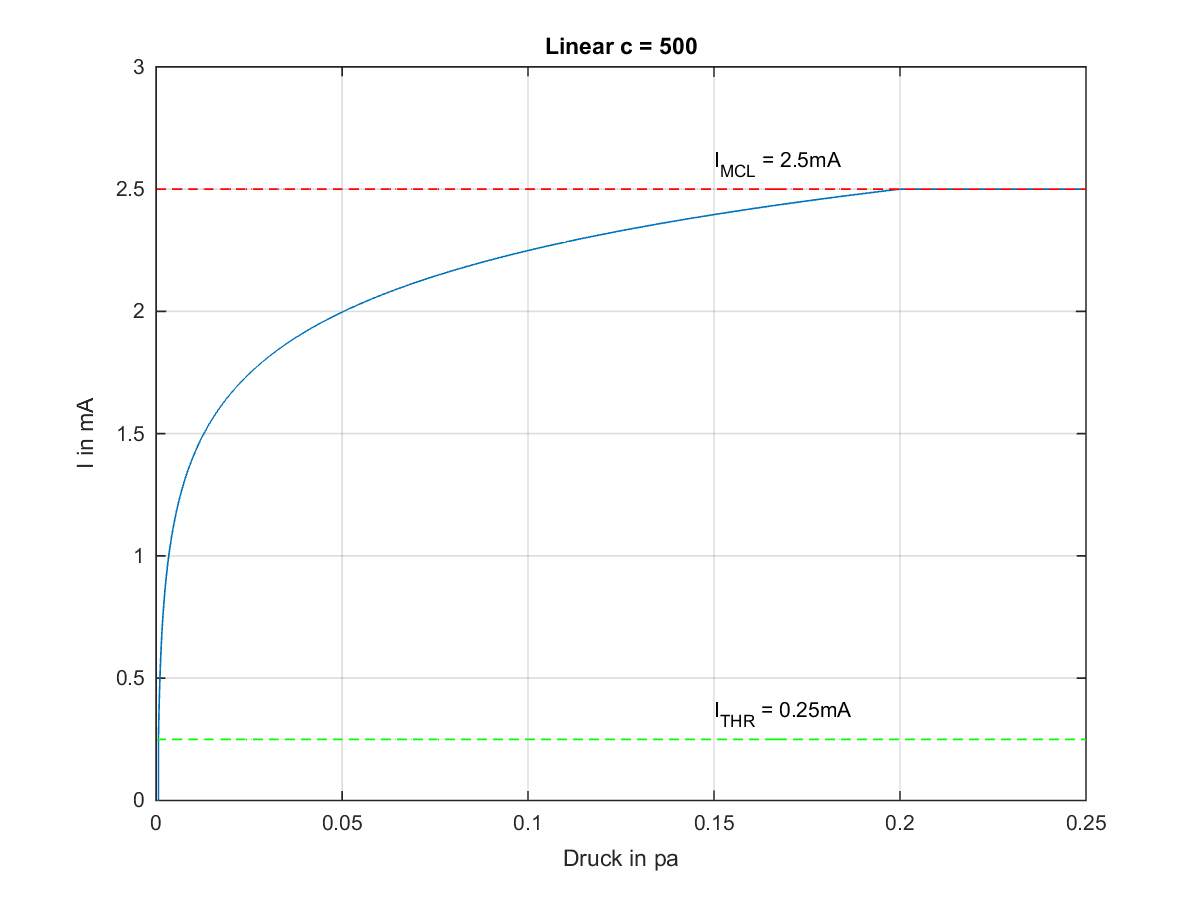
\includegraphics[width=0.5\textwidth]{img/lin_500.png}
	\vspace{-10pt}
	\caption{Kompressionskennlinie Linear mit Kompressionsrate 500}
	\vspace{-10pt}
	\label{fig:lin_500}
\end{figure}
\begin{figure}[h!]
	\centering
	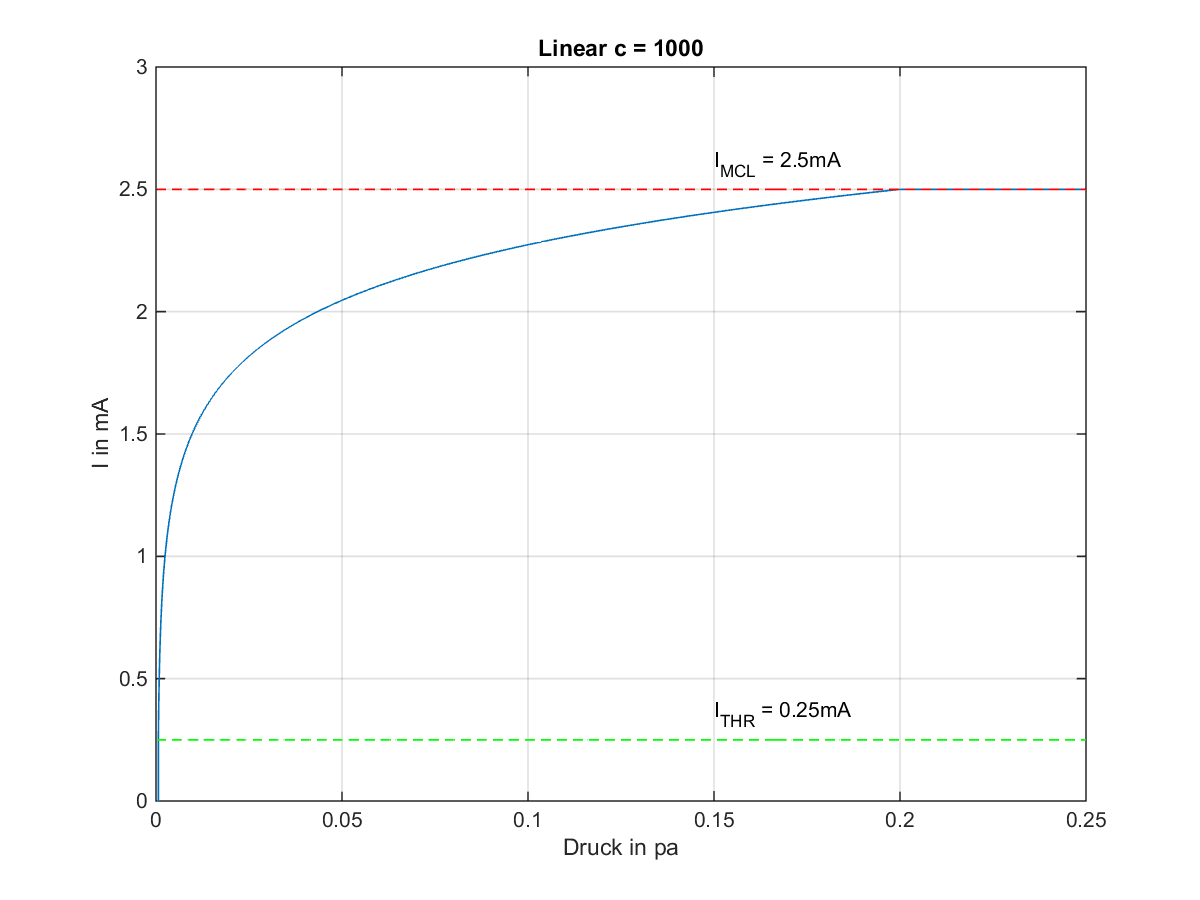
\includegraphics[width=0.5\textwidth]{img/lin_1000.png}
	\vspace{-10pt}
	\caption{Kompressionskennlinie Linear mit Kompressionsrate 1000}
	\vspace{-10pt}
	\label{fig:lin_1000}
\end{figure}

\begin{figure}
	\centering
	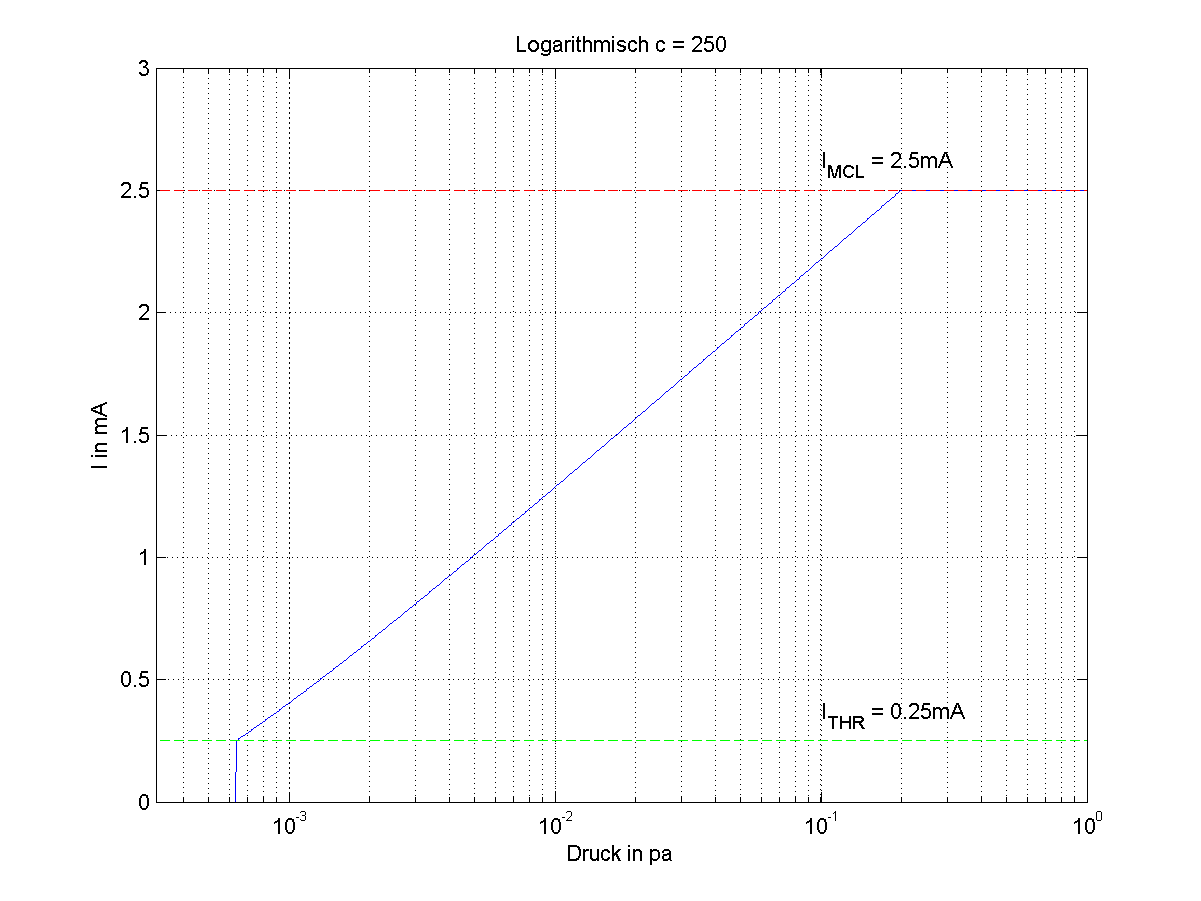
\includegraphics[width=0.5\textwidth]{img/log_250.png}
	\vspace{-10pt}
	\caption{Kompressionskennlinie Logarithmisch Linear mit Kompressionsrate 250}
	\vspace{-10pt}
	\label{fig:log_250}
\end{figure}
\begin{figure}[h]
	\centering
	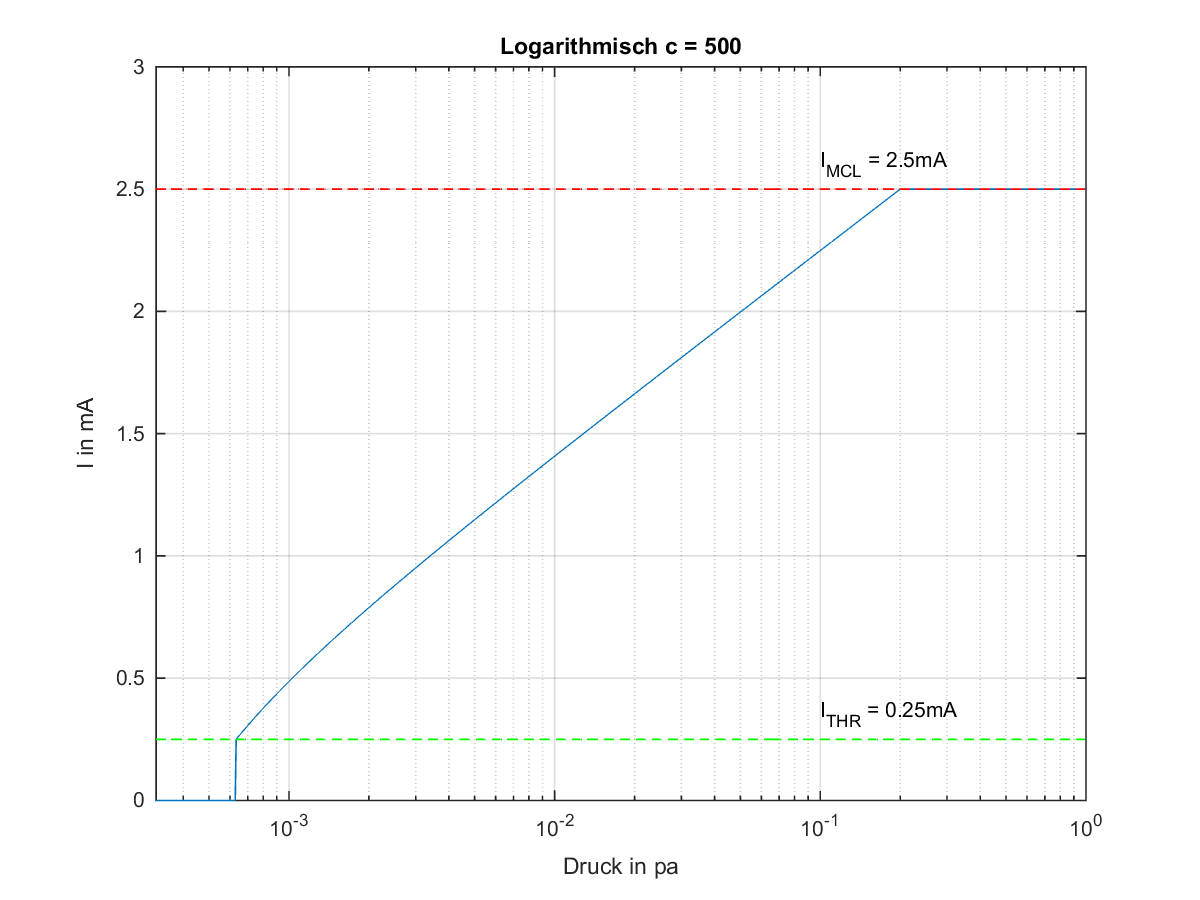
\includegraphics[width=0.5\textwidth]{img/log_500.png}
	\vspace{-10pt}
	\caption{Kompressionskennlinie Logarithmisch Linear mit Kompressionsrate 500}
	\vspace{-10pt}
	\label{fig:log_500}
\end{figure}
\begin{figure}[h!]
	\centering
	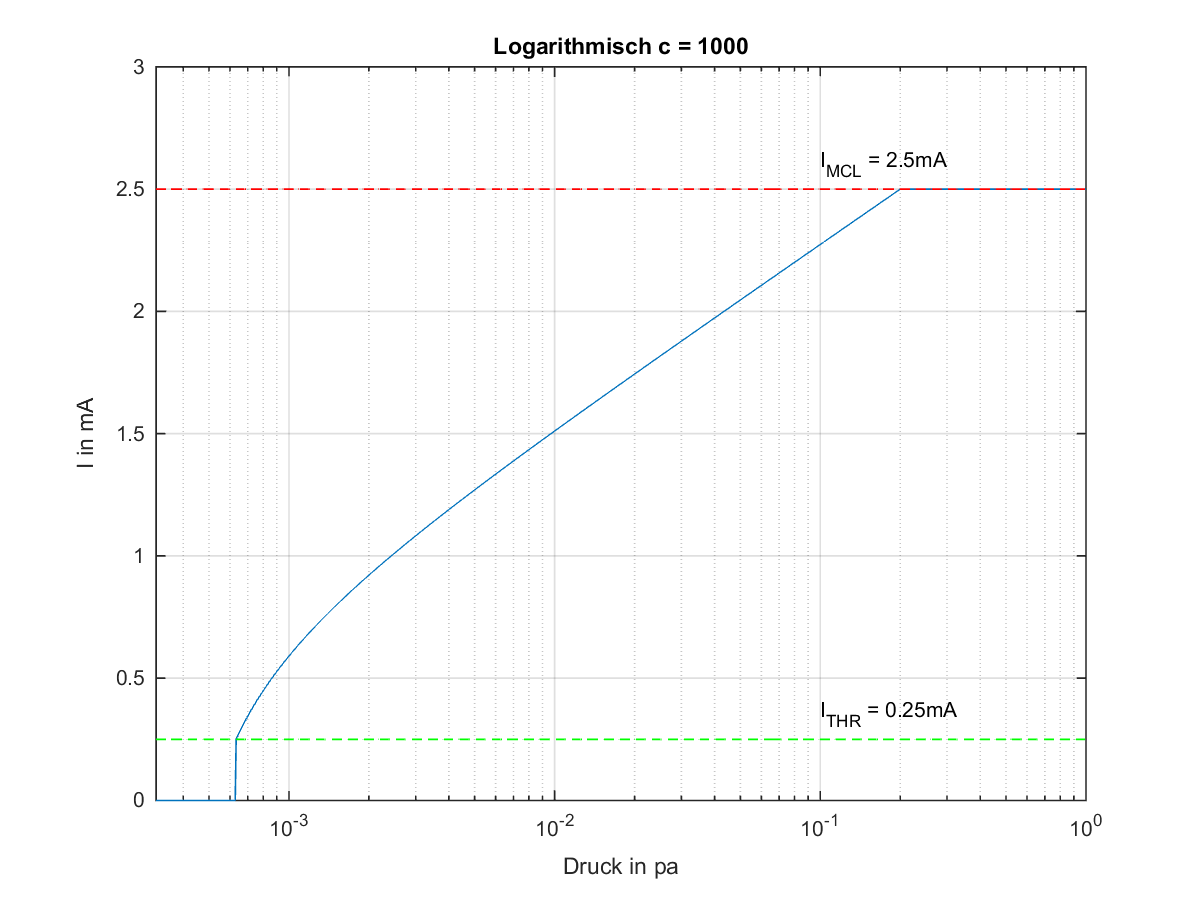
\includegraphics[width=0.5\textwidth]{img/log_1000.png}
	\vspace{-10pt}
	\caption{Kompressionskennlinie Logarithmisch Linear mit Kompressionsrate 1000}
	\vspace{-10pt}
	\label{fig:log_1000}
\end{figure}
\end{compactenum}

\end{document}


